\documentclass[twocolumn, prl]{revtex4}

\usepackage{amsmath}    % need for subequations
\usepackage[pdftex]{graphicx}   % need for figures
\usepackage{verbatim}   % useful for program listings
\usepackage{color}      % use if color is used in text
\usepackage{subfigure}  % use for side-by-side figures
\usepackage{hyperref}   % use for hypertext links, including those to external documents and URLs


\begin{document}

\title{The Fluid Dynamic Origin of Mammalian Ultrasonic Vocalizations}

\author{Matthew Dornfeld}
\email{mdornfe1@gmail.com}
\affiliation{Rockefeller University}

\author{Diego Laplagne}
\affiliation{Rockefeller University}

\author{Martin Costa} 
\affiliation{Rockefeller University}

\author{Marcelo Magnasco}
\affiliation{Rockefeller University}
\date{\today}
\begin{abstract}
Look, Dave … I can see you’re really upset about this … I honestly think you ought to sit down calmly … take a stress pill and think things over … I know I’ve made some very poor decisions recently, but I can give you my complete assurance that my work will be back to normal.
\end{abstract}
\maketitle
Although the purposes of animal vocalizations are staggeringly numerous, the apparatus by which they are produced seems to be largely conserved across mammal and bird species. This apparatus consists of membranous vocal fold tissues stretch across the larynx (or syrinx in birds). This tissue attaches to laryngeal muscles, which can alter its tension and degree of adduction. When air is forced past them by the lungs, the vocal folds oscillate and emit audible sounds, the frequency of which are determined by the vocal fold tension. Across species, the fundamental frequencies of audible mammalian vocalizations, which span several orders of magnitude in mass, obey a power law of the form $f\propto M^{-0.4}$, where M is the species mass in kg. However, many species of the orders Rodentia and Cetacia are known to produce narrowband ultrasonic whistles and broadband ultrasonic clicks, in addition to their sonic vocalizations. While the sonic vocalizations obey the aforementioned scaling law well, ultrasonic calls from the same species completely shatter the power law fit by over and order of magnitude (Figure \ref{fig:frequencye_scaling}). There is currently some debate over the exact nature of these ultrasonic calls, and the divergence from the scaling law is indicative that the production mechanism is fundamentally different from that of audible vocalizations \cite{Fletcher2010, Berke2010}.

%explain the broader implications of a physical model
Of the above mentioned ultrasonic vocalizations, the broadband clicks are believed to serve noncommunicative echolocative purposes. In odontocetes, the broadband clicks are known to be produced by a structure, called the phonic lips, which strike the fatty tissue of a structure called the melon, which transmits the vibrations to the surrounding water. However, The production mechanism behind the narrowband calls in cetaceans is currently uncertain. Furthermore, they are believed to be directed to conspecifics for the purpose of communication. Thus, the study of these vocalizations has broader implications for the fields of animal communication and ethology as a whole \cite{Reidenberg2010}. In rodents, some experimental work has been done, which discounts the possibility the narrowband calls are produced by vibrating vocal folds and indicates the production mechanism is a proper fluid dynamic whistle. However, there still does not exist a full quantitative theory of their production. It is for these reasons, this paper focuses on the narrowband rodent calls and aims to provide the beginnings of a quantitative theory of their production by fitting recordings of narrowband vocalizations to a fluid dynamic whistle model. This analysis is done with the hope that the study of narrowband rodent calls will provide greater insight into those of cetaceans \cite{Riede2011,Riede2011a,Roberts1975}.
\begin{figure}
\begin{center}
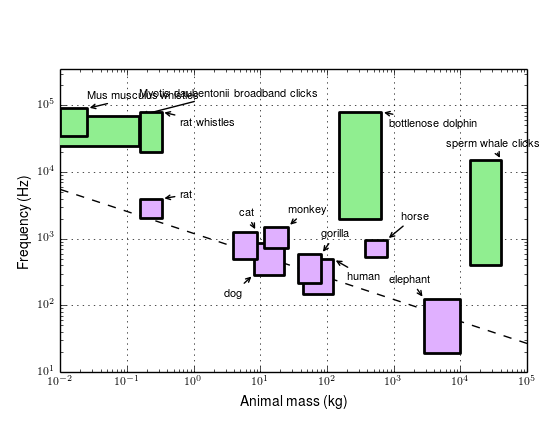
\includegraphics[width=\columnwidth]{frequency_scaling.png}
\caption{\label{fig:frequency_scaling} Frequency scaling law for mammalian vocalizations of the form $f\propto M^{-\alpha}$, where the dotted line is a theoretical relationship based on the conjecture that frequency should be proportional to cube of the linear scale of the animal. Thus, $\alpha=\frac{1}{3}.$ The solid line is gathered from experimental evidence across species and has $\alpha=0.4$ \cite{Brudzynski2010,White1998,berry1970natural,Fenton1998,Jones2006,bogdanowicz1994,Frankel2009,Whitehead2009}.}
\end{center}
\end{figure}



To fit data to this model, we examined the frequency jumps points from thousands of recorded calls from eleven different rats (nine male and two female). These recordings were obtained by sampling calls at 250-300 kHz using a condenser ultrasound Avisoft-Bioacoustics CM16/CMPA-5V microphone connected to a National Instruments data acquisition card. The recordings were then divided into call snippets based on long quiescence times between vocalizations. Afterwards the reassigned spectrogram of each call snippet was computed. Since each vocalizations is largely monotonal, a curve can be fitted to the call in time-frequency space by finding the frequency with the most power and computing the average of the seven frequency points surrounding and including that maximum- weighted by the amount of power in each frequency (see Figure \ref{fig:specgram}).This is done for each time point. Jump points can then be determined by finding points where the curve rapidly changes value. For each jump point, the after frequency can be plotted against the before. The data naturally groups itself into clusters along straight lines. Thus, we have extracted features with drastically lower dimensionality than the original data, and we hypothesize that each cluster corresponds to one type of mode transition, with $n\rightarrow n\pm1$. 
\begin{figure}
\begin{center}
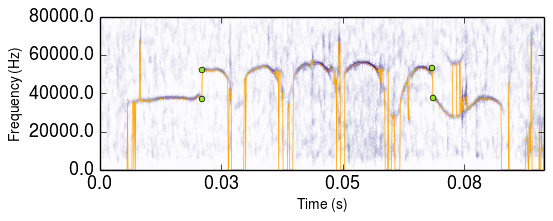
\includegraphics[width=\columnwidth]{specgram.png}
\caption{\label{fig:specgram} Reassigned spectogram of a frequency jump in an ultrasonic rat vocalization. The figure also shows the output of the curve fitting and jump point extraction algorithms.}
\end{center} 
\end{figure}

To test this conjecture a clustering algorithm was developed. As input, the algorithm accepts a list of straight lines. It then iterates over each jump point in the dataset and computes the perpendicular distance of the point to each line, which is then assigned to the line for which this value is minimum. If $\left(f_{1},\: f_{2}\right)$ and $\left(n,\: n\pm1\right)$ are the frequencies and mode numbers before and after a jump respectively, by dividing the after jump frequency mode relation by the before jump relation, we get \begin{equation}
\frac{f_{2}}{f_{1}}=m(c,\theta)=\frac{n\pm1-\theta}{n-\theta},\label{eq:freqmode2}
\end{equation}
where $c$ is the cluster to which that jump has been assigned, and $\left(n,\: n\pm1\right)$ is a function of the cluster. Several mode transitions were experimented with to best fit the data. In the extracted jumps, we found transitions in mode numbers ranging from 2 to 6. The 1 mode seems to correspond to 22 kHz alarm calls, which do not exhibit jumps as often and therefore are not represented in our dataset. Not all rats in our study produced enough jumps in all mode regions to fit the data to our algorithm, so underpopulated modes were excluded for some rats. Equation \ref{eq:freqmode2} can then be used to generate the slopes needed as input for the algorithm. We can define a cost function that adds up the squares of the perpendicular distances of each point to their assigned line. Let $\Delta x_{i_{c}}=\left\vert f_{1,i_{c}}-\frac{f_{1,i_{c}}+m\left(c,\theta\right)\left(f_{2,i_{c}}-b\right)}{m\left(c,\theta\right)^{2}+1}\right\vert $ be the $x$ distance from data point $i_c$ to the line and $\Delta y_{i_c}=\left\vert f_{2,i_{c}}-\frac{m\left(c,\theta\right)\left(f_{1,i_{c}}+m\left(c,\theta\right)\left(f_{2,i_{c}}-b\right)\right)}{m\left(c,\theta\right)^{2}+1} - b \right\vert$, the corresponding $y$ distance. 
\begin{equation}
C\left(\theta, b\right)=\sum_{c}\frac{1}{N_{c}}\sum_{i_c=1}^{N_{c}}\left(\Delta x_{i_c}\right)^{2}+\left(\Delta y_{i_c}\right)^{2},\label{eq:cost}
\end{equation}
where $N_{c}$ is the number of points in cluster $c$. We have also added an intercept parameter $b$ to allow for the possibility the best fit lines do not pass through the origin. By minimizing the cost function over $\theta$ and $b$ , we can get a determination for which cluster each point belongs to as well as a numerical calculation for the value $\theta$.

Figure \ref{fig:jumps} shows the output of the clustering algorithm, for each rat, for the values of $\theta$ and b that minimize the cost function, along with plots, for relevant values of n, of equation \ref{eq:freqmode2} with $\theta$ and b equal to those same values. The values of b are not shown here, since they were all found to be effectively zero, as expected. Figure \ref{fig:jumps}(a) shows an enlarged output of the clustering algorithm for one rat. For this rat, the data is grouped into eight clusters- four that correspond to up transitions and four that correspond to down transitions. This rat exhibits a significant number of jump points in the $2\rightarrow3$ and $3\rightarrow2$ transition clusters, which is somewhat rare, since these clusters are mostly populated by jumps between constant frequency calls in the 30 kHz range to constant frequency calls in the 50 kHz and vice versa, which were rarely recorded for an unknown reason. These clusters are noticeably distinct from the others and can be separated out by visual inspection. The clusters that represent transitions between higher regions present more of an overlap with each other. The $3\rightarrow4$, $5\rightarrow6$, $4\rightarrow3$, and $6\rightarrow5$ clusters show clear drop offs in density at their borders, which seems to be well represented in the output of the algorithm. However, the $4\rightarrow5$ and $5\rightarrow4$ transition clusters do not seem to be well represented in the data for this rat. Thus, it is hard to identify these clusters based on visual inspection of the density of jump points, although we still believe them to be present in smaller numbers. It is also worth noting that, removing those clusters from the algorithm did not produce a significant change in the calculated value of $\theta$. 

For each cluster, the ratio of after jump frequency to before jump frequency appears to be gaussianly distributed with mean approximately equal to the slope of each line that defines the cluster. Thus, the clustering algorithm accomplishes the task of separating out the overlapping density functions of each mode transition as well determining parameters for the whistle model that best fits the jump data. Figure \ref{fig:theta_error} shows the value of $\theta$ that minimizes equation \ref{eq:cost}, for each rat, along with the 95 \% confidence interval obtained from bootstrapping analysis. Since the jump points in Figure \ref{fig:jumps} fall along straight lines that can be separated in transition clusters, we can confidently conclude rat frequency jumps- and thus rat ultrasonic narrowband calls- are well explained by a whistle model. However, it can be seen that there is some variance in the values of $\theta$ obtained for each rat. Furthermore, they do not exactly agree with the published value of $\theta=0.25$ for hole tone whistles. However, this value was obtained with rigid boundaries and a jet that was perfectly aligned with the downstream aperture- both qualities we are unlikely to see in a biological system. Thus, we cannot conclude from Figure \ref{fig:theta_error} that ultrasonic whistles use a hole tone mechanism. However, considering the other results of this paper and the geometry of the rat vocal tract, this is likely the case. To verify this biologically accurate fluid dynamic simulations would need to be performed in an attempt to reproduce frequency jumps. 
\begin{figure*}
\begin{center}

\subfigure[]{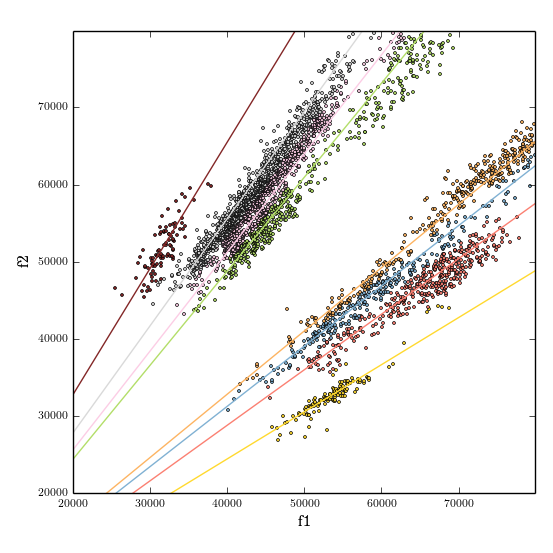
\includegraphics[width=\columnwidth]{V6.png}}
\subfigure[]{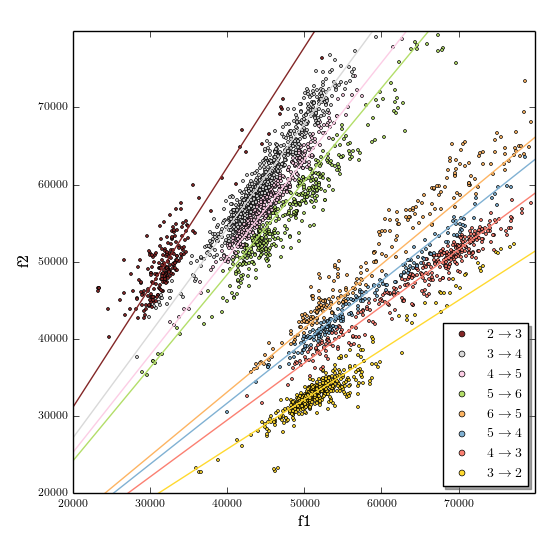
\includegraphics[width=\columnwidth]{V4.png}}
\caption{\label{fig:jumps}After jump frequency plotted against before jump frequency, along with plots of equation \ref{eq:freqmode2} for the mode number shown in the legend. For this rat, the data was best fit by four up clusters and four down clusters.} \end{center}
\end{figure*}
\begin{figure}
\begin{center}
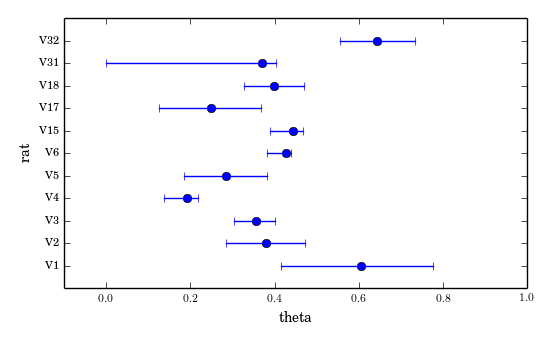
\includegraphics[width=\columnwidth]{theta_error_95.png}
\caption{\label{fig:theta_error}For each rat, the value of $\theta$ that minimizes equation \ref{eq:cost}, along with 95 \% confidence interval obtained from bootstrap analysis.} \end{center}
\end{figure}
\bibliographystyle{prsty}
\bibliography{mdornfe1.bib}
\end{document}